\chapter{Image Processing and Pattern Recognition}

In this chapter the image processing needed to pattern recognition and extract the exact QR-Code matrix. For this purpose, MATLAB is used, under the license provided by the University of Maryland College Park.


The procedure of detecting the image is explained in detail here and an excerpt of code script provided for better explanation. The overall flowchart for this section is as the image in the next page. The Reed-Solomon Decoder and message extraction box would be explained later. 


\tikzstyle{decision} = [diamond, draw, fill=blue!20, 
    text width=4.5em, text badly centered, node distance=3cm, inner sep=0pt]
\tikzstyle{block} = [rectangle, draw, fill=blue!20, 
    text width=5em, text centered, rounded corners, minimum height=4em]
\tikzstyle{line} = [draw, -latex']
\tikzstyle{cloud} = [draw, ellipse,fill=red!20, node distance=3cm,
    minimum height=2em]
    
\begin{tikzpicture}[node distance = 3cm, auto]
    % Place nodes
    \node [cloud] (expert) {Image};
    \node [block, below of=expert](init) {Image to binary};
    \node [cloud, right of=init, node distance=4cm] (system) {Version Num};
    \node [block, below of=init] (identify) {Median filter};
    \node [block, below of=identify] (evaluate) {Find three finder pattern};
    \node [block, left of=evaluate, node distance=4cm] (update) {Change im2binary threshold/Stop};
    \node [decision, below of=evaluate, node distance=4cm] (decide) {is there three finder pattern?};
    \node [block, below of=decide, node distance=4cm] (AP) {Find alignment pattern};
    \node [decision, right of=AP, node distance=5cm] (FindAP) {is there any alignment pattern?};
    
    \node [block, right of=FindAP, node distance=5cm] (Geo1) {Geo Trans using 3 FP and 1 AP};
    \node [block, below of=FindAP, node distance=5cm] (Geo2) {Geo Trans using 3 FP and the last corner};
    \node [block, above of=Geo1, node distance=3cm,text width=4cm] (Crop) {Extract the QR-Code exact image};
    \node [block, above of=Crop, node distance=4cm,text width=4cm] (FF) {Reed-Solomon Decoder/Message Extraction};
    % Draw edges
    \path [line] (init) -- (identify);
    \path [line] (identify) -- (evaluate);
    \path [line] (evaluate) -- (decide);
    \path [line] (decide) -| node [near start] {No} (update);
    \path [line,dashed] (update) |- (init);
    \path [line] (decide) -- node {Yes}(AP);
    \path [line,dashed] (expert) -- (init);
    \path [line,dashed] (system) -- (init);
    \path [line,dashed] (system) |- (evaluate);
    \path [line] (AP) -- (FindAP);
    \path [line] (FindAP) -- node{Yes}(Geo1);
    \path [line] (FindAP) -- node{No}(Geo2);
    \draw[ultra thick, blue, ->]  
    (Geo1) -- (Crop);
    \draw[ultra thick, blue, ->]  
    (Geo2) -- (Crop);
    \draw[ultra thick, red, ->]  
    (Crop) -- (FF);

   
\end{tikzpicture}


\section{Preprocessing}

\subsection{Image Transformation}

For the thresholding and creating a binary image, a sub-function named \textbf{$"im2binary\_Fn"$} has been design and implemented. This sub function get the image and using some thresholding return the black and white image. This is enough for QR-code because it only contains dark and bright modules which are binary $1$ and $0$ respectively. The script is as below:
\begin{lstlisting}
function Im_binary = im2binary_Fn(img,Thresh)
% Find the gray threshold level
if isempty(Thresh)
    Th = graythresh(img);
else
    Th = graythresh(img)-Thresh;
end
% Make the image binary using the level
Out = im2bw(img,Th);
Im_binary=Out;
\end{lstlisting}

\subsection{Median Filtering}

The reason of median filtering is that sometimes in the process of thresholding and creating a binary data from an image, patterns like salt and pepper noise might be produced. Median filtering is a powerful simple method to avoiding that flaw. The script is as simple as $ medfilt2(img)$. In order to better filtering one can use the different window sizes for the MATLAB function.

\section{Finding and Locating the Finder Patterns}

After thresholding and median filtering, the next task is to detect the QR code pattern from the image. For
this, we need to locate where the QR code is in the image and then reconstruct only the QR code part. The first major step is to finding three FPs\footnote{Finder Patterns}. According to the international
standard of QR code encoding \cite{1iso} and as we mentioned earlier, the ratio between the black and white modules in the
finder patterns is 1:1:3:1:1 which starts and ends with black. For finding finder pattern a horizontal and vertical search will be enough because from any point of view the aforementioned ratio is fixed with some tolerance coefficient. Sub-function $"find\_Probable\_FIPs\_Fn"$ use the following procedure for finding a finder pattern:

\textbf{Step1:}\\ Scan each row of the image and save the length of the black and white modules(How many successive pixels in a row have the same color). Sub-function $"Mod\_Tr\_Fn"$ detect the successive color order in a row matrix.

\begin{lstlisting}
for row = 1 : row_Num
        Tr_Line = img(row,:); % pick out the entire row
        
        % calculate the appearence of the modules in row.
        length_modules = Mod_Tr_Fn(Tr_Line);
end
\end{lstlisting}

Figure \ref{fig:3.1} demonstratess the row and column scanning.

\begin{figure}[H]
  \caption{Row and Column scanning for FPs locating}
  \centering
    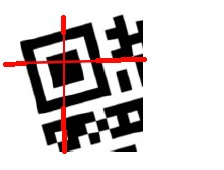
\includegraphics[width=0.5\textwidth]{figures/rowcolumnscan.jpg}
    \label{fig:3.1}
\end{figure}

\textbf{Step2:}\\ Consider every consecutive 5 elements of this length module of the row and calculate and extract the ratio of it.

\begin{lstlisting}
        for i = 1:length(length_modules)-4  
            vectorFIP = length_modules(i:i+4);
        end
\end{lstlisting}

\textbf{Step3:}\\ Check the ratio to see whether it is 1:1:3:1:1 or not. Also check to see that the first module is black or not. The sub-function $"checkRatio\_Fn"$ has been defined for checking the desired ration.

\begin{lstlisting}
[isFIP, ~] = checkRatio_Fn(vectorFIP, [1 1 3 1 1]);
            if(isFIP &&  img(row, pixelPosCol)==0)
\end{lstlisting}

\textbf{Step4:}\\ If the ratio is correct, the center position of the finder pattern which is the middle black block is found and save the length of the successive black and white modules in that column. Repeat step-2 and step-3 for the column.

\begin{lstlisting}
            if(isFIP &&  img(row, pixelPosCol)==0)
                col = pixelPosCol + floor(sum(vectorFIP)/2);
                pixelPosRow=1; %  Initial point
              
                Tr_col = Mod_Tr_Fn(img(:,col));
                 for j = 1:length(Tr_col)-4
                    vector_row_FIP = Tr_col(j:j+4);
                    [rowFIP, ~] =  checkRatio_Fn(vector_row_FIP, [1 1 3 1 1]);
                 end
                    
\end{lstlisting}




\textbf{Step5:}\\ One more time find the center position of the finder pattern in the column and check whether this point is over the previous center point or not. If the answer is yes so the center if found. If no, Ignore this row and check next row. 

\begin{lstlisting}
                    if(rowFIP && img(pixelPosRow,col)==0)
                        rows = pixelPosRow + sum(vector_row_FIP)/2;
                        if (abs(rows-row) <= 8) 
                            numberOfFIPS = numberOfFIPS + 1;
                            locationFIPs = [locationFIPs; [row col]];
                        end
                    end 
                    
\end{lstlisting}

\textbf{Note that the command $"if (abs(rows-row) <= 8)"$ is for a tolerance in coincidence of the row and column for finding the center}. We consider the number of 8. One can consider number of 1 for example. This factor if high let us consider more points as FIP candidates because is harsh situation which the image is very blurred or distorted, if the number of pixels is high even the finding of Finder Patterns would be difficult if the image is not straight because we cannot detect the correct ration.

\textbf{Step6:}\\ In the previous steps some finder patterns has been find as candidates. But we want to choose three of them which correspond to the main three finder patterns. The sub-function $"findFIP\_Order\_Fn"$ has been developed for doing that. The first part of it is to clustering which is an unsupervised learning using a famous pattern recognition MATLAB function which automatically divide the area into three category.

\begin{lstlisting}
    if( length(FIP) > 2 )

        [idx, Points] = kmeans(FIP,3,'Distance','cityblock',...
                           'Replicates',5)  ;    

        for i=1:3       
            Pos = Points(i,:);
            Determnd_Location = FIP(idx==i,:);       
            [~,index] =min( pdist2( Pos, Determnd_Location, 'euclidean') );
            FIPs(i,:)=Determnd_Location(index,:); 
        end
     end
                    
\end{lstlisting}

Then by searching the three cluster using the developed algorithm, three of them will be chosen. These three are the finder patterns.


\textbf{Step7:}\\ The last part is to extract the order of finder patterns because we now have the three finder patterns but we don't know which one is for example the top-left finder pattern or which one is the top-right. The sub-function $"get\_Correct\_Order\_FIPs\_Fn(FIPs)"$ in the last part of The sub-function $"findFIP\_Order\_Fn"$ performs this task. The following semi-pseudo code shows that:

\begin{lstlisting}
switch Max_indx
    Find A(pseudo code)
    AB = B-A;
    AC = C-A;
    %BC = C-B;
    k = AB(1)*AC(2) - AB(2)*AC(1);
    if k > 0
        C_point = C;
        B_point = B;
    else
        B_point = C;
        C_point = B;
    end
                    
\end{lstlisting}

Now lets have examples of finding finder patterns. the following figures show the locating of the finder pattern.
\begin{figure}[H]
  \caption{Finder pattern recognition of a damaged image}
  \centering
    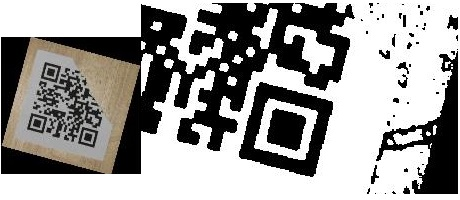
\includegraphics[width=0.9\textwidth]{figures/finderpattern1.jpg}
    \label{fig:3.2}
\end{figure}

\begin{figure}[H]
  \caption{Finder pattern recognition of QR-art}
  \centering
    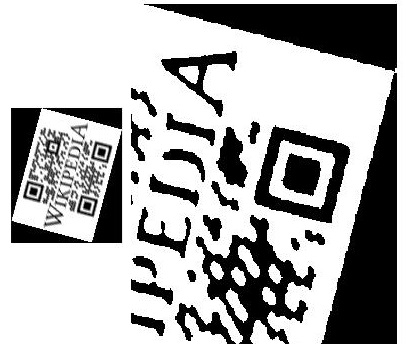
\includegraphics[width=0.9\textwidth]{figures/finderpattern2.jpg}
    \label{fig:3.3}
\end{figure}

\begin{figure}[H]
  \caption{Finder pattern recognition of distorted image}
  \centering
    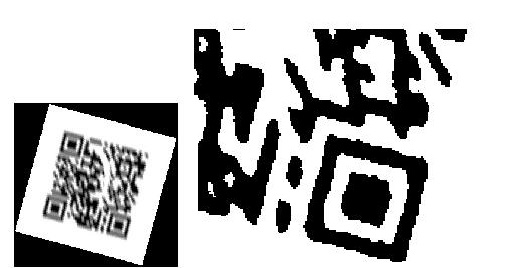
\includegraphics[width=0.9\textwidth]{figures/finderpattern3.jpg}
    \label{fig:3.4}
\end{figure}

\section{Finding the Alignment pattern Patterns}

After locating the finder patterns, the next task is to detect and locate the alignment pattern. For
this, we need to locate where the rounding area of AP\footnote{Alignment Pattern} is in the image and then search for the specific pattern. According to the standard of QR code \cite{1iso} the ratio between the black and white modules in the
AP is 1:1:1:1:1 which starts and ends with black. 

For finding finder pattern, in contrast with the FPs, a horizontal and vertical search will not be necessary enough because the algorithm may find such patterns in the image which are not any alignment patterns. Sub-function $"findAP\_Fn"$ use the following procedure for finding a finder pattern:

\textbf{Step1:}\\ The horizontal and vertical searching are exactly like the ones for locating finder patterns but the difference is that the ratio of 1:1:1 is considered to be searched. \textbf{Note that we do not search for ratio 1:1:1:1:1 because there is no separator for alignment pattern so we use the outer black square of the AP as a separator}.



\textbf{Step2:}\\ The previous step finds some candidates for being AP. This step performs a diagonal search for validating the candidates and ignore any candidate which does not have the ratio 1:1:1 from its diagonal point of view. Figure demonstrates the extra diagonal search. Sub-function $"check_AP_Fn"$ tries to validate different Alignment Patterns by diagonal search

\begin{lstlisting}
for i=1:size(locationAP,1)
    AP=locationAP(i,:);
    [ answer ] = check_AP_Fn( AP,img);
    if ~isempty(answer)
        APnew=[APnew;AP];
    end
end
                   
\end{lstlisting}

Sub-function $"check\_diag\_Fn"$ use the algorithm of diagonal search for checking the diagonal ratio.

\begin{lstlisting}
function answer = check_diag_Fn(AP,range,img)
Vec=[];
for i=-range:1:range
    Vec=[Vec img(AP(1,1)+i,AP(1,2)+i)];
end
length_modules = Mod_Tr_Fn(Vec);
c=1;
pos=[];
for k = 1:length(length_modules)-2
    row=sum(length_modules(1,1:k-1))+1;
    vectorAP = length_modules(k:k+2);
    [isAP, ~] = checkRatio_Fn(vectorAP, [1 1 1]);
    if (isAP && img(AP(1,1)-range+row-1,AP(1,2)-range+row-1)==1)
        pos(c) = sum(length_modules(1,1:k))+(length_modules(1,k+1))/2;
        c=c+1;
    end
end            
\end{lstlisting}

Basically we ignore the position if the radio of 1:1:1 cannot be detected there and/or the first module is not white(Remember that the black rounding square is used as separator).

Now its time to see some results. Recall that if the algorithm can find alignment pattern then it can plot it.

\begin{figure}[H]
  \caption{Finding Alignment pattern}
  \centering
    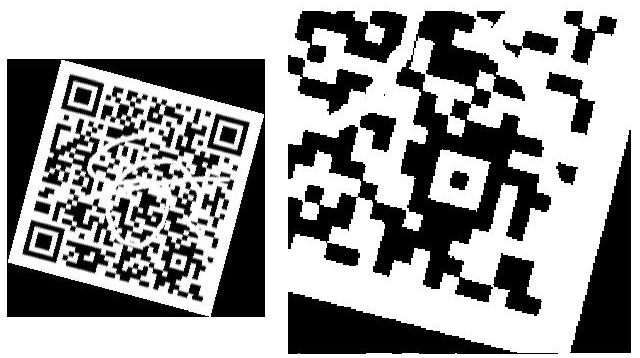
\includegraphics[width=0.9\textwidth]{figures/alignmentpattern1.jpg}
    \label{fig:3.5}
\end{figure}

\section{Geometric Modification}

Geometric Modification is necessary, since the image of the QR code may be distorted, blurred or damaged by any definition. The image must be deblurred and transformed a square pattern. At least 4-points(linearly independent) is needed to successfully perform geometric transformation. Two different approaches have been tried.

In the first approach, three finder pattern and the alignment pattern is used to geometrically transform the image. The approach has been developed for any version. But the necessary input is the version number. Figure \ref{fig:3.6} shows the approach.

\begin{figure}[H]
  \caption{Critical point detection}
  \centering
    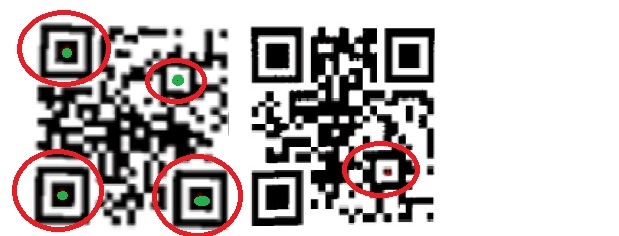
\includegraphics[width=0.9\textwidth]{figures/GeoAP.jpg}
    \label{fig:3.6}
\end{figure}

The next approach which is less precise compared to the previous one, is two find the fourth corner of the QR-code and use that point in staid of Alignment Pattern. This approached is applied when the algorithm cannot detect the center of Alignment Pattern which is possible in very distorted or blurred images.
By using the following code, the other extra points can be calculated and the fourth corner will be extracted to be used for perspective transformation.
\begin{lstlisting}
AC = C-A;
AB = B-A;
P=(B+C)/2;
    
% Find distance between the finder patterns
dist_1 = sqrt(AC(1)^2 + AC(2)^2);
dist_2 = sqrt(AB(1)^2 + AB(2)^2); 
% Difine as the new scale for QR-code reconstruction and is identical in both sides because QR-code pattern is square

cell_width_1=dist_1/(module-7);
cell_width_2=dist_2/(module-7);
normCA=unit_v_Fn(C,A);
normBA=unit_v_Fn(B,A);

%% Extra Points for better reflection
%% Four courners of A
    % A11-------A12
    % |    _/
    % |  _/
    % |_/
    % A21/-------A22

A11 = normCA*((module/2))*cell_width_1 + normBA*((module/2))*cell_width_2 + P;
A22 = normCA*((module/2)-7)*cell_width_1 + normBA*((module/2)-7)*cell_width_2 + P;
A12 = normAC*7*cell_width_1 + A11;
A21 = normAB*7*cell_width_2 + A11;

%% Four courners of B
    % B11-------B12
    % |    _/
    % |  _/
    % |_/
    % B21/-------B22
B11 = normAB*(module-7)*cell_width_2 + A11;
B21 = normAB*(module-7)*cell_width_2 + A21;
B12 = normAB*(module-7)*cell_width_2 + A12;
B22 = normAB*(module-7)*cell_width_2 + A22;

%% Four courners of C
    % C11-------C12
    % |    _/
    % |  _/
    % |_/
    % C21/-------C22

C11 = normAC*(module-7)*cell_width_1 + A11;
C21 = normAC*(module-7)*cell_width_2 + A21;
C12 = normAC*(module-7)*cell_width_2 + A12;
C22 = normAC*(module-7)*cell_width_2 + A22;


MM1= normAB*(module)*cell_width_2 + C12;% The last corener 
MM2= normAC*(module)*cell_width_1 + B21;        
\end{lstlisting}


\subsection{Perspective transformation}

The perspective transformation performs and describes the changes in a perspective projection, when the image is being looked from another point of view\cite{WikiHomo}. Using four point MATLAB can do the task directly. The following image demonstrates an example of perspective transformation.

\begin{figure}[H]
  \caption{Perspective Transformation\cite{StackPers}}
  \centering
    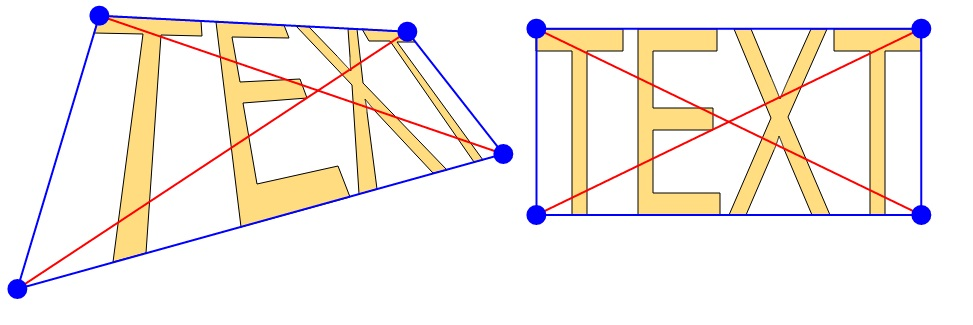
\includegraphics[width=0.9\textwidth]{figures/PersTrans.jpg}
    \label{fig:3.7}
\end{figure}

After finding 4-points which are not linearly dependent, Now we should define the corresponding 4-points to geometrically map the QR-code to a square image. Following code demonstrates the calculation which exactly defines the new corresponding points as "fixed points" and are the Finder patterns and Alignment Pattern places in the standard QR-Matrix which has been defined before.


\begin{lstlisting}

size(ap,2)
if (~isempty(ap) && module>21)      % Versions-1 may not have align pattern
moving_points = [fips(1,2) fips(1,1);            % B position
                    fips(2,2) fips(2,1);            % A position
                        fips(3,2) fips(3,1);        % C position
                            ap(2) ap(1);            % AP 
                            ];

fixed_points = [dist_min dist_fip;
                    dist_min dist_min;
                        dist_fip dist_min;
                              dist_ap dist_ap;
%                              (module)*cell_width (module)*cell_width;
%                              (7)*cell_width (7)*cell_width;
%                              (7)*cell_width (module-7)*cell_width;
%                              (module-7)*cell_width (7)*cell_width;
                            ];

end
       
\end{lstlisting}

Now its the time for MATLAB to transform the perspective by the following prepared function.
\begin{lstlisting}
tform = fitgeotrans(moving_points, fixed_points, 'projective');
newim_S = imwarp(Im, tform, 'linear');
\end{lstlisting}

\subsection{Crop and QR Pattern Demonstration}

After the previous steps, Now we need to crop the QR code pattern from the image and putting it in an exact square form. At first cropping is done by the following part of the program:

\begin{lstlisting}
rect = [FIPLocations(2,2)-(dist_min) FIPLocations(2,1)-(dist_min) side side];
newim = imcrop(newim, rect);
\end{lstlisting}

The using $"imresize"$ function and defining a bigger area(For better demonstration) the QR-code is extracted by the following part of the code:

\begin{lstlisting}
Main_QR_Matrix = imresize(newim, [module module], 'nearest');
Large_QR = imresize(Main_QR_Matrix, [10*module 10*module], 'nearest');
\end{lstlisting}

The following figures show the QR pattern final representation.

\begin{figure}[H]
  \caption{Version-3 QR code recognition}
  \centering
    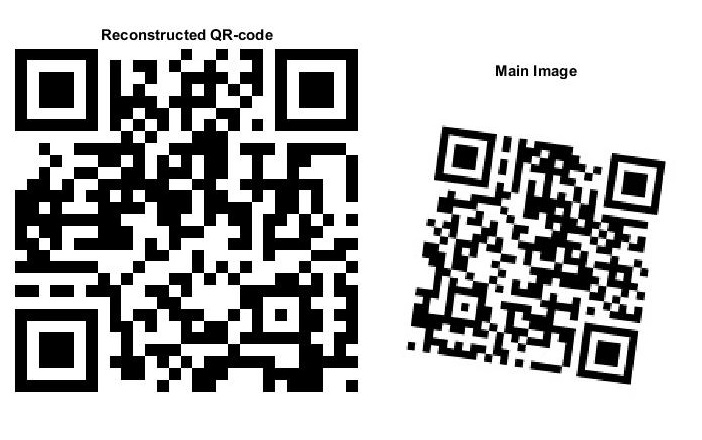
\includegraphics[width=0.9\textwidth]{figures/QR1.jpg}
    \label{fig:3.8}
\end{figure}

\begin{figure}[H]
  \caption{Verion-2 QR code}
  \centering
    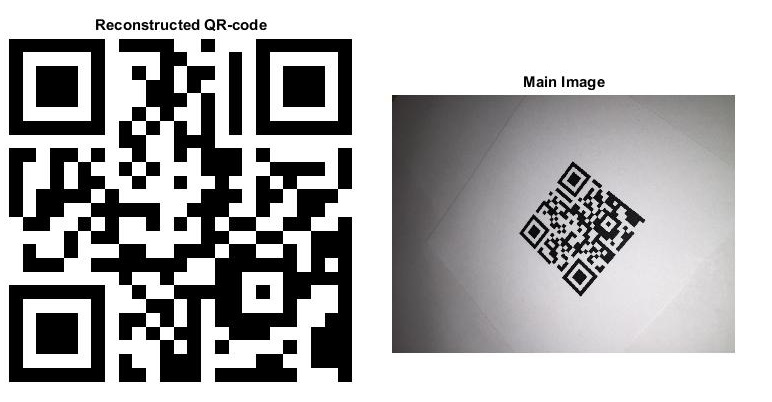
\includegraphics[width=0.9\textwidth]{figures/QR2.jpg}
    \label{fig:3.9}
\end{figure}

\begin{figure}[H]
  \caption{QR code recognition in a high resolution image}
  \centering
    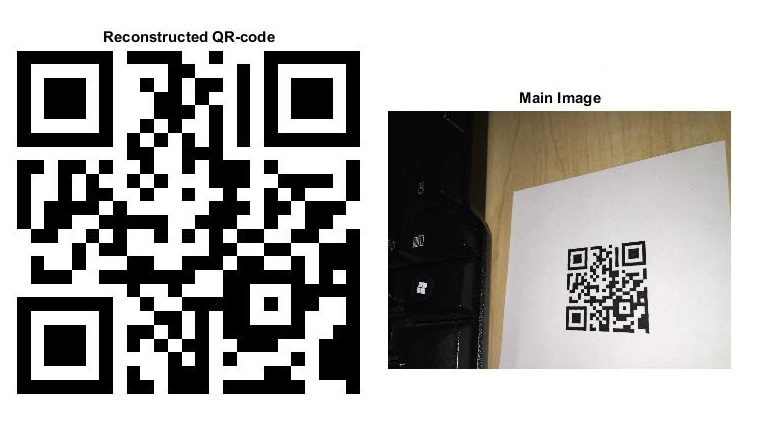
\includegraphics[width=0.9\textwidth]{figures/QR3.jpg}
    \label{fig:3.10}
\end{figure}


This chapter was dedicated to the Image Processing part of the project. In the next chapter decoding of the message will be discussed.







